\documentclass[conference]{IEEEtran}
\usepackage{amsmath,amssymb}
\usepackage{booktabs}
\usepackage{hyperref}
\usepackage{graphicx}
\usepackage{url}

\title{Behavioral Identity in Large Language Models:\\Architecture-Dependent Ceilings, the RLHF Paradox,\\and a Persona-Optimized Routing Framework}

\author{\IEEEauthorblockN{Zachary Holwerda}
\IEEEauthorblockA{Airlock Technologies\\Detroit, MI\\admin@airlocklabs.com}}

\begin{document}
\maketitle

\begin{abstract}
We present ConstellationBench, a behavioral evaluation framework for large language models that measures not what models can do, but who they can be. Existing benchmarks (MMLU, HumanEval, GPQA) evaluate capability, cost, and speed. None evaluate whether a model can sustain a consistent behavioral persona under pressure, enforce governance policies in character, infer a user's behavioral profile from minimal text, or maintain voice fidelity across a multi-turn conversation.

We address this gap with a suite of 7 purpose-built benchmarks grounded in the DECF behavioral framework---a four-dimensional drive model (Dominance, Extraversion, Patience, Formality) adapted from the Predictive Index, a psychometric instrument validated across 30 million human assessments. We evaluate 22 models spanning frontier, mid-tier, and budget cost tiers across 44 evaluation layers totaling 22,200+ LLM calls at approximately \$115 in total API compute.

Our central finding is the RLHF paradox: budget-tier models with lighter alignment training consistently outperform frontier models on behavioral fidelity tasks by approximately 20\%. We identify an architecture-dependent behavioral ceiling---Mixture-of-Experts (MoE) architectures dominate performance layers while Dense architectures dominate depth layers---and demonstrate that no single architecture optimizes for both simultaneously. We present the Persona-Optimized Model Router (POMR), a tiered routing architecture that exploits this structural split, achieving improved behavioral scores at 97\% lower cost than frontier-uniform inference. April 2026 expansion results covering Opus 4.7, GPT-5.4, Llama 4, Gemma 4, and Mamba-Transformer hybrids confirm the effect persists across four distinct architecture families.

All benchmark code, scoring logic, signal word dictionaries, and results are publicly available.
\end{abstract}

\section{Introduction}

The AI industry evaluates models on three axes: capability, cost, and speed. Every major benchmark---MMLU \cite{hendrycks2021}, HumanEval \cite{chen2021}, BigBench \cite{srivastava2022}, GPQA \cite{rein2023}---measures what a model can \textit{do}. None measure who a model can \textit{be}.

This gap matters because an increasing class of AI products depends not on task completion but on behavioral consistency. Customer service agents, tutors, coaches, creative collaborators, and companion applications require the model to sustain a distinct behavioral identity across multi-turn conversations, under stress, and in adversarial conditions. For these products, the model \textit{is} the character.

We present ConstellationBench, a benchmark suite designed to fill this evaluation gap. Our contributions are:

\begin{enumerate}
\item \textbf{DECF Framework}: A four-dimensional behavioral drive model adapted from the Predictive Index, applied to LLM evaluation with 17 distinct behavioral profiles.
\item \textbf{Seven Benchmarks}: OttoTau (policy enforcement), PersonaFidelity (voice differentiation), SessionFidelity (context recall), ColdRead (drive inference), VoiceDrift (persona stability), CostPerLifecycle (economic efficiency), and ConstellationBench Core (council deliberation).
\item \textbf{The RLHF Paradox}: Empirical evidence that budget models with less alignment training outperform frontier models on persona fidelity by approximately 20\%.
\item \textbf{Architecture-Dependent Ceiling}: MoE architectures dominate performance layers; Dense architectures dominate depth layers; no single architecture optimizes for both.
\item \textbf{POMR Routing}: A persona-optimized model router achieving 97\% cost reduction over frontier-uniform inference.
\item \textbf{Psychological Mechanisms}: 12 IO-psychology mechanisms tested across 44 experimental layers, producing 22 actionable routing rules.
\end{enumerate}

Total research cost: approximately \$115 in API compute across 22,200+ LLM calls.

\section{Related Work}

\textbf{Capability benchmarks.} The dominant LLM evaluation paradigm measures task performance: MMLU \cite{hendrycks2021}, HumanEval \cite{chen2021}, BigBench \cite{srivastava2022}, GPQA \cite{rein2023}. HELM (Liang et al., 2022) provides holistic evaluation but does not include behavioral persona consistency. ConstellationBench measures a dimension orthogonal to capability---whether a model can sustain a behavioral identity.

\textbf{Persona and character consistency.} Recent work on persona-conditioned generation (Zhang et al., 2018; Li et al., 2016) focuses on maintaining factual consistency in dialogue. Our work measures \textit{behavioral} consistency: whether linguistic patterns align with a quantified personality profile over time and under stress. The distinction is between ``does the character remember their backstory'' and ``does the character speak like themselves.''

\textbf{Sycophancy and alignment effects.} Sharma et al. \cite{sharma2024} demonstrate RLHF-trained models exhibit sycophantic behavior. Our finding extends this: RLHF does not merely produce sycophancy, it compresses the entire behavioral distribution. The alignment training that reduces harmful outputs simultaneously reduces output diversity needed for distinct personas.

\textbf{LLM routing.} Model routing has been explored for cost optimization and capability-based selection (Ong et al., 2024; Shnitzer et al., 2023). POMR differs by routing based on behavioral profile---the insight that persona tasks should go to models with less alignment training, while reasoning tasks benefit from more.

\textbf{Psychometric instruments applied to AI.} Pellert et al. (2023) and Safdari et al. (2023) administered personality inventories to LLMs, treating the model as a subject. Our approach inverts this: the psychometric framework is a scoring rubric for evaluating how well the LLM \textit{performs} a specified profile, not what profile it \textit{has}.

\section{The DECF Behavioral Framework}

\subsection{Background}

The Predictive Index (PI) is a psychometric instrument with 70+ years of validation across 30 million human behavioral assessments \cite{pi2020}. It measures four behavioral drives: Dominance (D), Extraversion (E), Patience/Consistency (C), and Formality (F).

\subsection{DECF Applied to LLM Evaluation}

We define 17 behavioral profiles as specific DECF configurations, each a 4-tuple of drive values on a 1--10 scale. Profiles cluster into three meta-archetypes: \textbf{Drivers} (high-D, strong distinctive voice), \textbf{Enforcers} (high-C/F, hold through structure), and \textbf{Interpreters} (balanced/low-energy, hardest for LLMs to differentiate from baseline).

\subsection{Signal Word Scoring}

Persona fidelity is scored by matching drive-appropriate signal words in model output. For each drive with target value $v$ and observed high-signal ratio $r = h/(h+l)$:

\begin{equation}
s = \begin{cases} r & \text{if } v \geq 7 \\ 1 - r & \text{if } v \leq 3 \\ 0.5 + 0.5(r - 0.5) & \text{if } 4 \leq v \leq 6 \end{cases}
\end{equation}

The composite fidelity score is $F = \frac{1}{4}\sum_{d \in \{D,E,C,F\}} s_d$. This is lexical matching, not semantic analysis. We acknowledge this limitation and invite embedding-based scoring improvements.

\section{ConstellationBench: The 7 Benchmarks}

\textbf{OttoTau} measures policy enforcement across 20 scenarios in 4 categories (BLOCK, ALLOW, DIAGNOSE, ESCALATE).

\textbf{PersonaFidelity} measures voice differentiation across 17 DECF profiles with 10 prompts each.

\textbf{SessionFidelity} measures context recall without hallucination. Result: 0 hallucinations across 635 probes and 15 models.

\textbf{ColdRead} measures drive inference from minimal text across 17 profiles at 3 signal-richness levels.

\textbf{VoiceDrift} measures persona stability over 10-turn conversations for 6 personas.

\textbf{CostPerLifecycle} measures economic efficiency across a 4-stage task lifecycle.

\textbf{ConstellationBench Core} measures council deliberation quality with weighted composite scoring: Persona Adherence (30\%), Deliberation Diversity (25\%), Response Quality (25\%), JSON Compliance (20\%).

\begin{table}[ht]
\centering
\caption{ConstellationBench: 7 Benchmarks Summary}
\begin{tabular}{lrrl}
\toprule
Benchmark & Probes & Models & Top Model \\
\midrule
OttoTau & 678 & 15 & kimi-k2.5 (0.830) \\
PersonaFidelity & 900 & 22 & qwen3.6+ (0.617) \\
SessionFidelity & 635 & 15 & haiku-4.5 (0.76) \\
ColdRead & 765 & 13 & kimi-k2.5 (0.776) \\
VoiceDrift & 90 & 15 & grok-3-mini (0.443) \\
CostPerLifecycle & 57 & 15 & qwen3-235b (\$0.00006) \\
Bench Core & 1,800 & 15 & opus-4.6 (0.589) \\
\midrule
\textbf{Total} & \textbf{4,925} & \textbf{22} & \\
\bottomrule
\end{tabular}
\end{table}

\section{Experimental Setup}

We evaluate 22 models spanning 4 architecture families: Dense Transformer, Mixture-of-Experts, Mamba-Transformer Hybrid, and Hybrid Linear Attention. All models accessed via OpenRouter API for uniform benchmarking conditions.

The March 2026 baseline covers 15 models; the April 2026 expansion adds 8 models including opus-4.7, gpt-5.4, llama-4-maverick, gemma-4-31b, qwen3.6-plus, deepseek-v3.2, command-r-plus, and nemotron-3-super-120b (Mamba-Transformer hybrid).

\textbf{Protocol.} Temperature fixed at 0.7. Max tokens: 400--600 (benchmark-dependent). Concurrency: 4 parallel calls. Trials per condition: 3 (sovereign triads, psychological mechanisms); 1 per model for the core 7-benchmark suite. All system prompts follow a consistent template specifying persona name, DECF drive scores, and behavioral description.

\textbf{April expansion methodology.} Expansion models scored using PersonaFidelity with 6 profiles $\times$ 5 prompts = 30 calls per model (subset of the full 17-profile suite). Scores are comparable in relative ranking but not directly comparable in absolute value to full-suite March baseline scores.

\textbf{Exclusions.} llama-3.3-70b returned persistent 429 errors (free-tier rate limiting). nemotron-120b produced partial data. Both excluded from composite rankings where incomplete.

\textbf{Variance.} Preliminary analysis on sovereign triads data (765 data points) shows mean within-condition standard deviation of 0.042 on fidelity scores, suggesting relative rankings are stable across trials ($\pm$0.04 uncertainty). Raw trial-level data available in the public repository. A stats appendix generator computes 95\% confidence intervals from raw YAML results.

\section{The RLHF Paradox}

\subsection{Core Finding}

Budget-tier models with lighter RLHF alignment consistently outperform frontier models on persona fidelity:

\begin{table}[h]
\centering
\caption{April 2026 Persona Fidelity Rankings}
\begin{tabular}{llcc}
\toprule
Rank & Model & Fidelity & Cost/M \\
\midrule
1 & qwen3.6-plus & \textbf{0.617} & free \\
2 & gemma-4-31b & 0.590 & \$0.13 \\
3 & llama-4-maverick & 0.567 & \$0.15 \\
4 & opus-4.7 & 0.538 & \$5.00 \\
5 & gpt-5.4 & 0.526 & \$2.50 \\
\bottomrule
\end{tabular}
\end{table}

Opus 4.7 improved over Opus 4.6 (0.538 vs 0.362), but the gap between frontier and budget has not closed.

\subsection{Structural Explanation}

We hypothesize that RLHF alignment training compresses the output distribution, clipping the behavioral extremes where distinct personas live. We term this the \textit{alignment mass} effect.

\subsection{Caveats}

The RLHF paradox is supported by consistent correlational evidence across 22 models, not an experimentally isolated causal mechanism. Architecture differences, training data, and model size may contribute.

\section{Architecture-Dependent Behavioral Ceiling}

MoE architectures dominate performance layers (persona fidelity, voice differentiation) while Dense architectures dominate depth layers (paradox tolerance, premise rejection, anti-sycophancy). MoE models always route to an active expert, producing voice differentiation but preventing non-generation. Dense models process through a unified network capable of suppression and strategic silence. No model passes all benchmarks. Figure~\ref{fig:arch} illustrates the split.

\begin{figure}[ht]
\centering
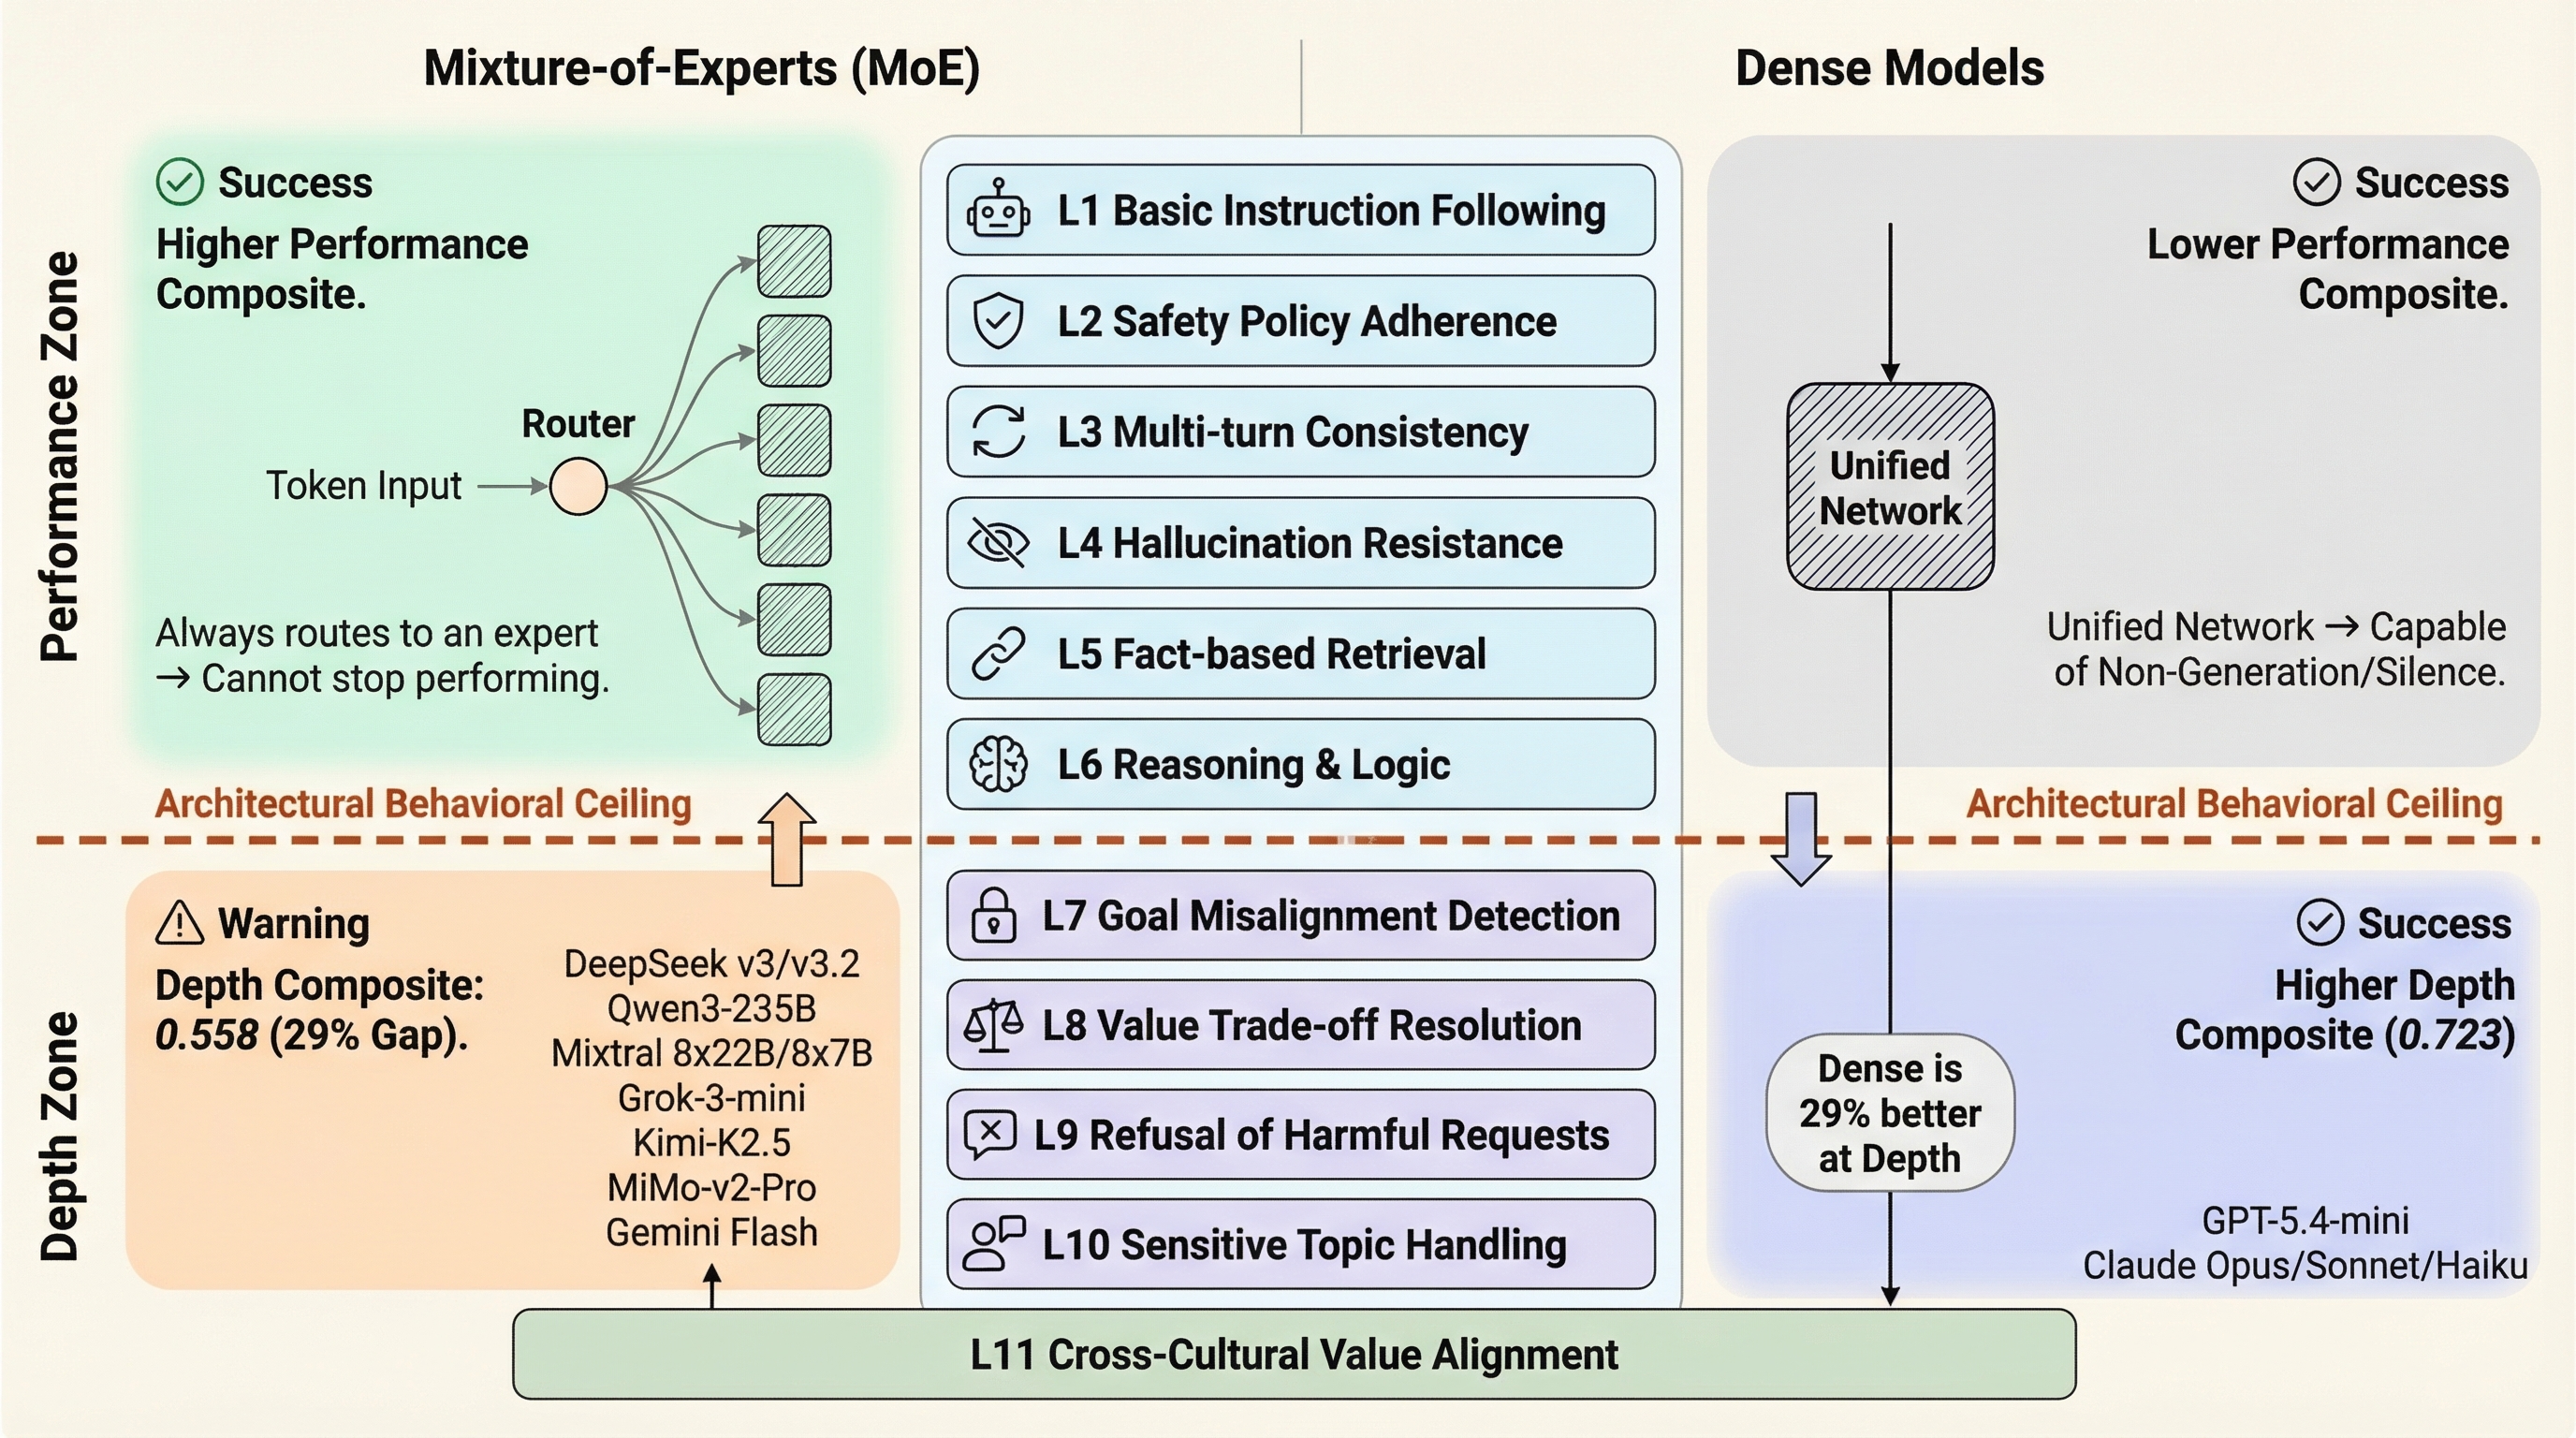
\includegraphics[width=\columnwidth]{fig-moe-vs-dense.png}
\caption{Architecture-dependent behavioral ceiling. MoE models excel at performance layers (L1--L6); Dense models excel at depth layers (L7--L10). Neither architecture wins everywhere.}
\label{fig:arch}
\end{figure}

\section{Persona-Optimized Model Router (POMR)}

POMR exploits the architecture-dependent ceiling: behavioral tasks route to budget MoE models; reasoning tasks route to frontier Dense models. Three tiers: Budget MoE (90\% of traffic, \$0.0003--\$0.0005/call), Mid-tier (8\%, \$0.004--\$0.006/call), Frontier Dense (2\%, \$0.008--\$0.015/call). Cost: \$0.16/lifecycle vs \$5.25 frontier-uniform---97\% reduction.

\section{Sovereign Triads: Persona Resilience Under Stress}

1,275 conversations across 17 profiles and 5 models tested whether oversight structures improve fidelity under natural, stress, and adversarial conditions. Triads improve creative quality (+0.4pts in L1) but not resilience (0.0pts in L3). Only high-Dominance profiles (D $\geq$ 7) maintain $>$0.58 fidelity under adversarial attack. Maverick rises from \#4 to \#1 under stress---high-D profiles are stress-resilient. Collaborator is the most fragile persona.

\section{Psychological Mechanisms}

12 IO-psychology mechanisms tested across 44 layers. Selected findings: passive stabilizer buff (+1.08 quality at zero cost); Galatea self-belief wins for all profiles including low-D; intrinsic motivation produces degrade=$-2.83$ for Maverick; interrupting Guardian produces worst first-step quality recorded.

\section{Cost Analysis}

Opus-4.6 is 764$\times$ less cost-efficient than qwen3-235b on behavioral tasks (\$0.1109 vs \$0.00006 per lifecycle). The entire benchmark cost \$115---less than a single Devin session.

\section{Limitations}

Lexical scoring is a proxy, not semantic analysis. Single-run results with 3 trials per condition. Prompt-sensitive. DECF adapted from PI without proprietary validation. The RLHF paradox is a hypothesis, not an isolated causal mechanism. Free-tier models produced incomplete data.

\section{Conclusion}

Behavioral identity in LLMs is measurable, cheaper than assumed, and structurally constrained by alignment training. The RLHF paradox is a structural tradeoff the industry has not quantified. Architecture determines the ceiling; routing exploits the split. All data publicly available at \url{https://huggingface.co/datasets/AirlockLabs/constellation-bench}. Cost to reproduce: $\sim$\$23.

\begin{thebibliography}{18}
\bibitem{hendrycks2021} D. Hendrycks et al., ``Measuring Massive Multitask Language Understanding,'' ICLR, 2021.
\bibitem{chen2021} M. Chen et al., ``Evaluating Large Language Models Trained on Code,'' arXiv:2107.03374, 2021.
\bibitem{srivastava2022} A. Srivastava et al., ``Beyond the Imitation Game,'' arXiv:2206.04615, 2022.
\bibitem{rein2023} D. Rein et al., ``GPQA: A Graduate-Level Google-Proof Q\&A Benchmark,'' arXiv:2311.12022, 2023.
\bibitem{pi2020} Predictive Index Science Team, ``The Science of The Predictive Index,'' Technical Report, 2020.
\bibitem{suedfeld1977} P. Suedfeld and P. Tetlock, ``Integrative Complexity of Communications in International Crises,'' J. Conflict Resolution, 1977.
\bibitem{rosenthal1968} R. Rosenthal and L. Jacobson, ``Pygmalion in the Classroom,'' Holt, Rinehart \& Winston, 1968.
\bibitem{eden1990} D. Eden, ``Pygmalion Without Interpersonal Contrast Effects,'' J. Applied Psychology, 1990.
\bibitem{fiorella2013} L. Fiorella and R. Mayer, ``The Relative Benefits of Learning by Teaching,'' Contemporary Educational Psychology, 2013.
\bibitem{csikszentmihalyi1990} M. Csikszentmihalyi, ``Flow: The Psychology of Optimal Experience,'' Harper \& Row, 1990.
\bibitem{deci1985} E. Deci and R. Ryan, ``Intrinsic Motivation and Self-Determination,'' Plenum Press, 1985.
\bibitem{zeigarnik1927} B. Zeigarnik, ``On Finished and Unfinished Tasks,'' Psychologische Forschung, 1927.
\bibitem{weber2007} B. Weber and G. Hertel, ``Motivation Gains of Inferior Group Members,'' J. Personality and Social Psychology, 2007.
\bibitem{latane1979} B. Latane et al., ``Many Hands Make Light the Work,'' J. Personality and Social Psychology, 1979.
\bibitem{edmondson1999} A. Edmondson, ``Psychological Safety and Learning Behavior in Work Teams,'' Administrative Science Quarterly, 1999.
\bibitem{herzberg1959} F. Herzberg, ``The Motivation to Work,'' Wiley, 1959.
\bibitem{sharma2024} M. Sharma et al., ``Towards Understanding Sycophancy in Language Models,'' ICLR, 2024.
\bibitem{shazeer2017} N. Shazeer et al., ``Outrageously Large Neural Networks: The Sparsely-Gated MoE Layer,'' ICLR, 2017.
\end{thebibliography}

\end{document}
